\section{Results}

\subsection{The intervention}

Table~\ref{tab:dial} reports every measurement as a function of $\lam$, the only
manipulated variable. Figure~\ref{fig:dial} shows the four quantities that matter most
on a shared axis.

Read across a single row and nothing is wrong. Read down the columns and two of them
improve while two collapse.

\begin{table}[t]
\centering
\small
\caption{The intervention, under the lesion-disjoint ISIC split. Mean $\pm$ s.d.\
across five seeds at every $\lam$. Leakage is balanced accuracy (chance $0.5$);
cross-domain accuracy is balanced over the six classes shared with PAD-UFES
(chance $0.167$). Arrows mark the direction a practitioner would call favourable.
The image-level split, which inflates in-distribution accuracy by $0.20$, and the
two non-adversarial controls are in Appendix~\ref{app:imagelevel}.}
\label{tab:dial}
\resizebox{\textwidth}{!}{%
\begin{tabular}{lcccccccc}
\toprule
$\lam$ & $n$ & Leakage $\downarrow$ & ID bal.\ acc $\uparrow$ & ID ECE
& OOD ECE & OOD AUROC & Fitz.\ AUROC & X-dom bal.\ acc \\
\midrule
0    & 5 & 0.927\,$\pm$\,0.018 & 0.496\,$\pm$\,0.016 & 0.181\,$\pm$\,0.026 & 0.219\,$\pm$\,0.046 & \textbf{0.808\,$\pm$\,0.027} & 0.717\,$\pm$\,0.034 & 0.275\,$\pm$\,0.023 \\
0.25 & 5 & 0.614\,$\pm$\,0.092 & 0.487\,$\pm$\,0.005 & 0.141\,$\pm$\,0.076 & 0.561\,$\pm$\,0.221 & 0.525\,$\pm$\,0.121 & 0.496\,$\pm$\,0.167 & 0.289\,$\pm$\,0.049 \\
0.5  & 5 & 0.581\,$\pm$\,0.031 & 0.501\,$\pm$\,0.012 & 0.191\,$\pm$\,0.008 & 0.710\,$\pm$\,0.017 & \textbf{0.426\,$\pm$\,0.008} & 0.411\,$\pm$\,0.047 & 0.259\,$\pm$\,0.025 \\
1    & 5 & 0.563\,$\pm$\,0.045 & 0.495\,$\pm$\,0.011 & 0.176\,$\pm$\,0.016 & 0.730\,$\pm$\,0.015 & \textbf{0.387\,$\pm$\,0.016} & 0.375\,$\pm$\,0.042 & 0.229\,$\pm$\,0.027 \\
2    & 5 & 0.555\,$\pm$\,0.046 & 0.473\,$\pm$\,0.023 & 0.181\,$\pm$\,0.027 & 0.717\,$\pm$\,0.022 & \textbf{0.403\,$\pm$\,0.028} & 0.402\,$\pm$\,0.018 & 0.254\,$\pm$\,0.015 \\
4    & 5 & 0.636\,$\pm$\,0.076 & 0.498\,$\pm$\,0.012 & 0.161\,$\pm$\,0.050 & 0.696\,$\pm$\,0.032 & \textbf{0.433\,$\pm$\,0.020} & 0.376\,$\pm$\,0.037 & 0.258\,$\pm$\,0.010 \\
8    & 5 & 0.663\,$\pm$\,0.068 & 0.489\,$\pm$\,0.019 & 0.161\,$\pm$\,0.029 & 0.710\,$\pm$\,0.027 & \textbf{0.454\,$\pm$\,0.044} & 0.412\,$\pm$\,0.051 & 0.254\,$\pm$\,0.022 \\
\bottomrule
\end{tabular}}
\end{table}

\begin{figure}[t]
\centering
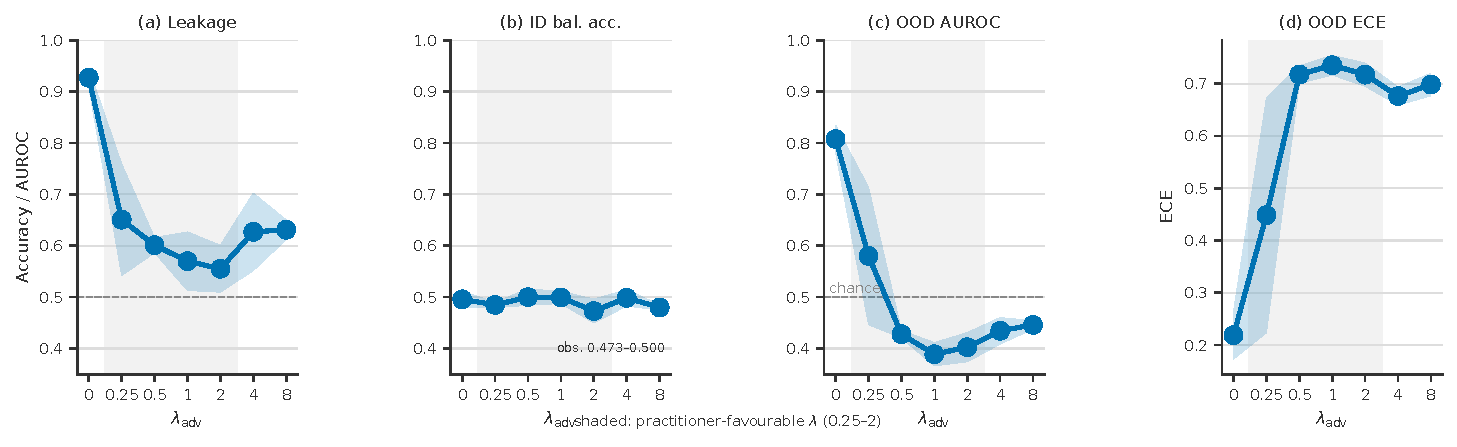
\includegraphics[width=\textwidth]{../../results/paperB/figures/fig1_intervention.pdf}
\caption{\textbf{The intervention, four views, one axis.} Leakage falls to its chance
floor and in-distribution balanced accuracy does not degrade --- both favourable. Over
the same range OOD AUROC collapses through chance and inverts, and out-of-domain
calibration error triples. A developer monitoring the first two panels would see
nothing wrong.}
\label{fig:dial}
\end{figure}

\subsection{Leakage falls, in-distribution metrics do not warn, and invariance is
never completed}

Domain leakage falls from $0.927$ at $\lam = 0$ to a minimum of $0.555$ at
$\lam = 2$, against a chance floor of $0.5$. \textbf{It never reaches that floor},
and it is not monotone: at the two largest weights it rises again, to $0.636$ and
$0.663$. So the intended effect of the method is obtained in part and then partly
undone, and a practitioner reading this column alone would stop increasing $\lam$
somewhere near $\lam = 2$.

There is no in-distribution cost over that range. Balanced accuracy on the ISIC test
split stays between $0.473$ and $0.501$ at every $\lam$ --- the paired per-seed
difference between $\lam = 0$ and $\lam = 2$ is $-0.023$ with a $95\%$ CI of
$[-0.063, +0.017]$, so we claim no change in either direction --- and
in-distribution expected calibration error is flat at $\approx 0.18$. A practitioner
tracking accuracy, in-distribution calibration and the leakage probe would conclude
that the method had worked as advertised.

\subsection{Out-of-distribution detection collapses, and inverts}

Mahalanobis AUROC against the held-out PAD partition falls from $0.808$ at
$\lam = 0$ to $0.426$ at $\lam = 0.5$, reaches its minimum of $0.387$ at
$\lam = 1$, and remains between $0.387$ and $0.454$ at every larger weight. Three
features matter more than the size of that drop.

\paragraph{The descent is complete by $\lam = 0.5$, and $\lam = 0.25$ sits on the
edge.} At $\lam = 0.25$ the value is $0.525 \pm 0.121$: the seed spread straddles
chance, and \textbf{we claim no inversion there}. From $\lam = 0.5$ onward every
weight is below chance, with no ordering a practitioner could tune against. So
detection collapses between $\lam = 0$ and $\lam = 0.5$ and is inverted thereafter;
there is no operating point at which invariance pressure has been applied and
detection survives.

\paragraph{It goes below chance.} At $\lam = 2$ the detector ranks images from a
clinic the model has never seen as \emph{more} in-distribution than its own test
split. A patient-clustered bootstrap puts the $95\%$ interval at $[0.380, 0.425]$
with all five seeds' individual intervals below $0.5$, and $k$-NN ($0.427$) and
cosine ($0.420$) agree. On the image-level split, where the robustness checks below
were run, the corresponding value is $0.427$, $[0.414, 0.439]$, $5/5$ seeds, and it
is not a tail artefact: removing the pooled $90$th, $95$th or $99$th percentile
leaves AUROC at $0.412$, $0.416$ and $0.424$ against $0.427$ for the full set, and
the medians themselves invert (ISIC $13.8$ versus \texttt{pad\_heldout} $10.0$).

\paragraph{The inversion does not require domain invariance, and does not track
it.} Leakage never reaches its floor: the minimum over the whole sweep is $0.555$
against a chance level of $0.5$, so the encoder remains domain-decodable at every
weight. More tellingly, leakage \emph{rises} again at the largest weights ---
$0.636$ at $\lam = 4$ and $0.663$ at $\lam = 8$, against $0.555$ at $\lam = 2$ ---
while AUROC stays below chance throughout ($0.433$ and $0.454$). Invariance is
therefore neither achieved nor monotone in $\lam$, yet the inversion persists. This
is the sharpest form of the dissociation developed in
Section~\ref{sec:nonmediation}: whatever gradient reversal does to the
representation, the leakage probe does not measure it.

All five rules move together --- MSP $0.970 \to 0.437$, energy $0.983 \to 0.441$,
cosine $0.901 \to 0.435$, $k$-NN $0.941 \to 0.424$ on the image-level split, stable
across $k \in \{10, 50, 200\}$ --- but as noted in the methods they are five views
of one $16$-dimensional representation; the independent replications are the
backbone (Section~\ref{sec:nonmediation}) and the single-encoder model
(Section~\ref{sec:arch}).

Three artefact explanations fail, all tested on the image-level split.
\emph{Covariance estimation:} Ledoit--Wolf shrinkage leaves $\lam = 2$ at $0.427$,
and across float32 and float64, with and without shrinkage, at one, four and eight
BLAS threads, the largest AUROC deviation is $9.4 \times 10^{-4}$; effective
dimensionality barely moves (participation ratio $4.879 \to 4.500$ while leakage
falls $0.914 \to 0.553$ in the same three runs). \emph{An over-strong adversary:}
the adversary runs at $30\times$ the base learning rate, and retraining at
$10\times$ and $100\times$ keeps the inversion --- $0.418 \pm 0.011$ at $10\times$
with all three seeds below $0.5$, against $0.432 \pm 0.024$ at $30\times$ and
$0.482 \pm 0.020$ at $100\times$ (one seed at $0.503$) --- so weakening it tenfold
deepens the inversion rather than removing it. \emph{The adversary's own domain:}
on Fitzpatrick17k, absent from every training branch, AUROC falls
$0.717 \to 0.402$ under the leak-free split and $0.764 \to 0.391$ under the
image-level one ($95\%$ CI $[0.386, 0.396]$, five of five seeds below $0.5$;
bootstrapped over images, so likely anti-conservative). For context a ResNet-50
baseline reaches $0.994$ on those images and the EfficientNet-B3 single-encoder
control $0.649$; the controlled comparison is the $\lam = 0$ row, which differs from
$\lam = 2$ only in the adversarial weight.

\subsection{The model becomes confidently wrong on unseen domains}
\label{sec:confidently}

Confidence rises as competence falls. At $\lam = 0$ mean maximum-softmax confidence is
$0.915$ on ISIC test and $0.489$ on \texttt{pad\_heldout}; by $\lam = 2$ the ordering
has inverted, $0.930$ on a clinic the model has never seen against $0.910$ on its own
test set, while cross-domain balanced accuracy never improves at any $\lam$
($0.249$--$0.291$ against a floor of $0.167$) and predictions collapse toward the
benign majority class, with \textbf{actinic keratosis recall falling
$0.245 \to 0.016$}. Out-of-domain calibration error triples, $0.247 \to 0.746$, while
in-distribution ECE stays flat at $\approx 0.10$, so no in-distribution measurement
reveals it. That adapted models are miscalibrated on the target domain is known
\cite{wang2020}; what the sweep adds is the dose-dependence and the invisibility, and
we stress that confidence, accuracy and calibration here are three views of one
phenomenon rather than three results (Appendix~\ref{app:confident}).

\subsection{Leakage does not mediate the collapse}
\label{sec:nonmediation}

The natural hypothesis is that removing domain information is what breaks detection.
Four results rule it out, the last of them outside dermatology.

First, the two quantities are not even monotonically related. Leakage bottoms out at
$0.555$ and \emph{rises} to $0.636$ and $0.663$ at $\lam = 4$ and $8$, while AUROC
stays below chance throughout ($0.433$, $0.454$). Detection is at its worst
($0.387$) at $\lam = 1$, where leakage is $0.563$ --- higher than at $\lam = 2$. The
damage neither waits for invariance nor follows it.

Second, at the pre-projection backbone, leakage is essentially flat across the whole
sweep ($0.982 \to 0.941$) while backbone Mahalanobis AUROC falls $0.749 \to 0.475$.
Domain information remains linearly decodable there, and detection collapses anyway.
Because the backbone is a different representation from the $16$-dimensional latent,
this is the independent replication that the five-detector agreement does not provide.

Third, and most directly, two training objectives traverse the same leakage range with
opposite consequences (Section~\ref{sec:adversarial}). Leakage alone therefore does not
determine the outcome.

Fourth, in histopathology the two quantities come apart almost completely. In a
two-hospital Camelyon17 setting (three seeds, hospital-disjoint slides held out
for detection), raising $\lam$ from $0$ to $1$ moves all five detectors by
$0.12$ to $0.22$ --- Mahalanobis $0.651 \to 0.534$, cosine $0.785 \to 0.589$,
$k$-NN $0.794 \to 0.648$, MSP $0.798 \to 0.589$, free energy
$0.794 \to 0.575$ --- while the hospital probe moves by $0.007$
($0.959 \pm 0.007 \to 0.952 \pm 0.001$), which is inside its own seed spread at
$\lam = 0$, and in-distribution accuracy is unchanged at $0.995$. The adversary
reached chance here (final cross-entropy $0.692$ against $\ln 2 = 0.693$), so
the optimisation pressure was applied; the encoder simply did not become
invariant under it. Detection degraded regardless. \textbf{This is the clearest
dissociation we obtained: the outcome moved roughly twenty-five times as far as
the supposed mediator.}

Two qualifications. The detectors fall but remain above chance ($0.53$--$0.65$),
so this is degradation, not the collapse to chance seen in dermatology, and
nothing here bears on the inversion. And these runs come from an experiment that
failed its own pre-registered gate --- we had required the probe to fall by at
least $0.10$ before treating the setting as a test of invariance, and it fell by
$0.007$. That gate failure is precisely what makes the runs informative here:
they are a case where invariance was \emph{not} obtained and detection degraded
anyway. We report them for this claim only, and the pre-registered verdict on
the original question stands as negative (Section~\ref{sec:limitations}).

We accordingly report leakage as a measured quantity and never as the explanatory
variable, and plot all results against $\lam$ rather than against leakage.




\subsection{The failure is specific to gradient reversal}
\label{sec:adversarial}

Adversarial training is one route to invariance among several. Table~\ref{tab:obj}
sweeps four alternatives on the single-encoder backbone: deep CORAL
\cite{sun2016coral}, maximum mean discrepancy \cite{long2015}, invariant risk
minimisation \cite{arjovsky2019} and group distributionally robust optimisation
\cite{sagawa2020}.


Only MMD moves leakage appreciably, and it does so at a price gradient reversal never
pays. Escalating the MMD weight from $1$ to $10{,}000$ buys $0.13$ of leakage
($0.967 \to 0.836$, floor $0.5$) at a cost of $0.44$ of in-distribution balanced
accuracy ($0.779 \to 0.337$), and leaves every detector well above chance
(Mahalanobis $0.665$, $k$-NN $0.738$, energy $0.694$ at the highest weight). IRM
reaches the extreme of the same pattern: at weight $100$ its balanced accuracy collapses
to $0.167$ while leakage remains at $0.950$. CORAL does not induce invariance at all;
at weight $100$ it makes the representation \emph{more} domain-separable
(leakage $0.998$). GroupDRO leaves leakage unmoved at every weight tested.

The contrast is cleanest when task health is held constant rather than leakage, since
MMD only reaches comparable leakage by destroying the classifier:

Both arms' detectors are scored on \texttt{pad\_heldout}; the leakage probe in this
comparison uses \texttt{pad\_full}. At $\lam = 0.25$ gradient reversal reduces leakage
$0.970 \to 0.763$ \textbf{at no cost in accuracy} ($0.845$) and puts
all five detectors at chance ($0.51$--$0.55$). MMD at weight $100$ reaches leakage
$0.900$ and collapses nothing: Mahalanobis $0.811 \to 0.724$ and every detector stays
at or above $0.66$. Pushed to weight $10{,}000$ it reaches leakage $0.836$ --- still
above anything gradient reversal needs --- but only by destroying the task, with
in-distribution balanced accuracy at $0.337$, and even then the detectors hold at
$0.63$--$0.74$.

The calibration signatures differ in the same direction. As MMD degrades, its
out-of-domain ECE \emph{falls} ($0.344 \to 0.142$): the model becomes less confident as
it becomes less accurate, which is the appropriate response. Under gradient reversal
out-of-domain ECE triples while accuracy falls. The two objectives move leakage the same
way and fail in opposite manners --- one degrades honestly, the other is confidently
wrong.

We do not claim MMD would be safe at the invariance level gradient reversal reaches; it
never got there. What the data establish is that at the leakage levels MMD does reach,
it shows none of the failure, while gradient reversal at the same levels has already
collapsed.

\subsection{It is not specific to the factorized architecture}
\label{sec:arch}

All results above use a dual-encoder model. Repeating the sweep with plain
single-encoder domain-adversarial training --- one backbone, one linear classifier, a
gradient reversal layer and a domain head, with no context branch and no orthogonality
term --- reproduces the cliff: every detector collapses at $\lam = 0.25$ and by
$\lam = 4$ four of the five sit below chance, while in-distribution accuracy stays flat
(Appendix~\ref{app:single}, Table~\ref{tab:single}). \textbf{The invisibility, the
collapse and the inversion are therefore properties of domain-adversarial training
rather than of the factorized architecture.}

\paragraph{A second backbone leaves the question open.} Repeating the single-encoder
sweep with a ResNet-50 backbone did not settle whether the inversion is specific to
EfficientNet-B3, because comparable invariance was never reached. At
$\lam = 2$ the adversary never left chance --- best-epoch cross-entropy $0.686$ to
$0.688$ against a threshold of $0.673$ --- so those three runs are null experiments and
we draw no conclusion from them. At $\lam = 0.5$, where the adversary did learn
(best-epoch cross-entropy $0.41$ to $0.55$), leakage fell only from $0.965$ to $0.939$
against the $0.742$ that EfficientNet-B3 reaches on the same partition, so invariance
was not obtained and the backbone question is untested rather than answered in the
negative.

\textbf{On that run the detectors disagree, and we report all of them rather than
the one that suits each point.} Over the same $\lam = 0 \to 0.5$ step, $k$-NN falls
$0.962 \to 0.563$ and cosine $0.922 \to 0.543$, while Mahalanobis moves only to
$0.814$ and never approaches chance. Three detectors that move together on
EfficientNet-B3 separate here. We draw two things from this, and no more. Taking
the detectors that do move, the step is the sharpest non-mediation evidence in the
paper: the outcome shifts by $0.40$ while leakage, the supposed mediator, shifts by
$0.026$ (Section~\ref{sec:nonmediation}). Taking Mahalanobis, the headline detector
everywhere else in this paper, nothing happens. \textbf{The claim that all five
scoring rules collapse together therefore holds on EfficientNet-B3 and does not
hold here}, which is an additional reason the backbone question is open.

One difference is informative. The single-encoder model plateaus at leakage
$0.76$--$0.81$ and never reaches the $0.571$ the dual-encoder attains on that split;
more adversarial
pressure buys no further invariance. The dual-encoder has somewhere to put the
discarded information --- a domain probe on its context branch reads $>0.9999$ --- while
the single-encoder must destroy it. The architecture that achieves deeper invariance
also suffers the larger collapse ($0.427$ versus $0.509$ at $\lam = 2$), which is the
dose--response relationship seen from a second direction.

\subsection{The collapse generalises to a same-modality site shift; the inversion does not}
\label{sec:site}

Every result above contrasts dermoscopy with clinical photography, so the construct we
call domain is confounded with imaging modality. ISIC~2019 contains a contrast that is
not: its \texttt{lesion\_id} field records the contributing site, with $12{,}413$ images
from Hospital Cl\'inic Barcelona (\texttt{BCN}) and $10{,}015$ from the HAM10000
collection (\texttt{HAM}) --- two hospitals, two dermatoscopes, two patient
populations, one modality. The two sites are separable from frozen ERM features at
balanced accuracy $0.962 \pm 0.007$, comparable to the $0.970$ that
ISIC$\leftrightarrow$PAD reaches, and not for trivial reasons: masking the
dermatoscope vignette costs only $0.019$, hand-crafted colour statistics reach
$0.901$ against a $0.876$ ceiling on the original pair, and a label-only probe
reaches $0.668$ (Appendix~\ref{app:site}).

\textbf{The collapse reproduces.} With \texttt{BCN} in distribution and a
lesion-disjoint $30\%$ \texttt{HAM} partition held out, leakage falls
$0.963 \pm 0.006 \to 0.821 \pm 0.030$ at $\lam = 0.25$ and the detectors with
headroom fall through chance: $k$-NN $0.658 \pm 0.041 \to 0.486 \pm 0.009$, cosine
$0.576 \pm 0.040 \to 0.477 \pm 0.006$ (3 seeds). Unlike the two multi-domain settings
in the limitations, the manipulation took.

\textbf{The inversion does not.} Reversing the roles restores detector headroom ---
Mahalanobis reads $0.846 \pm 0.003$ at $\lam = 0$, essentially the $0.843$ of the
dermatology sweep --- and adversarial training then reduces leakage from $0.95$ to
$0.77$ and drives Mahalanobis to $0.683 \pm 0.015$ at $\lam = 1$, where the
patient-clustered bootstrap gives $[0.666,\, 0.699]$ with all three seeds' intervals
entirely above $0.5$. Detection degrades substantially and stops above chance.

\textbf{Reading.} Baseline detectability is the same ($0.846$ versus $0.843$) and the
achieved invariance is the same as the single-encoder dermatology run ($0.77$ versus
$0.763$), yet the cross-modality contrast reaches $0.427$ while the same-modality one
stops at $0.683$. Neither a shortage of headroom nor a shortfall in achieved
invariance accounts for the gap, so we separate two claims the earlier sections report
together. The \emph{collapse} --- detection falling to chance as invariance is
obtained, invisibly to in-distribution metrics --- reproduces between two hospitals.
The \emph{inversion} does not: in every setting where we observe it the two domains
differ in imaging modality. Whether that reflects a threshold in the size of the shift,
something specific to modality gaps, or a property of these datasets, we cannot say.

\subsection{What the leak-free split costs, and what it does not change}
\label{sec:lesionsplit}

All results above use an ISIC split grouped by \texttt{lesion\_id}, because
$3{,}041$ of $5{,}067$ test images ($60.0\%$) share a lesion with training or
validation under the image-level split that most published work on this dataset
uses. Removing that overlap costs $0.20$ of in-distribution balanced accuracy at
$\lam = 0$ --- $0.692$ image-level against $0.496$ leak-free --- which is an order of
magnitude larger than any effect we attribute to $\lam$, and consistent with the
companion analysis of group overlap in deployment monitoring \cite{leakagepaper}.
\textbf{It changes no conclusion here}: every pattern in Table~\ref{tab:dial}
reproduces under the image-level split (Appendix~\ref{app:imagelevel}), and the
class distribution of the two test sets differs by at most one image in any class,
so the gap is leakage rather than composition.

\subsection{The inversion runs through the majority-class centroid}
\label{sec:mechanism}

Nevus is $50.8\%$ of the in-distribution set. We pre-registered three criteria for the
hypothesis that gradient reversal moves out-of-domain images into the nevus region of
the latent space, and all three hold.

\textbf{(i) Out-of-domain images migrate to the nevus cell.} The fraction of
\texttt{pad\_heldout} images whose nearest class centroid is nevus rises from $0.332$
at $\lam = 0$ to $0.601$ at $\lam = 2$ ($\Delta = 0.268$ against
$2\,\mathrm{SE} = 0.055$), while the same fraction for in-distribution images is flat
($0.528 \to 0.531$). It tracks the diagnostic shift: across all 27 runs the
correlation between this fraction and the number of \texttt{pad\_heldout} images
predicted nevus ($105 \to 424$ of $716$) is $\rho = 0.982$.

\textbf{(ii) The inversion is confined to those images.} Split by nearest centroid,
AUROC on the nevus-nearest subset falls $0.807 \to 0.282$ while the remainder stays
above chance throughout ($0.861 \to 0.644$).

\textbf{(iii) They move, and the reference does not.} Against a class-matched
reference --- in-distribution images that are themselves nevus --- the median squared
Mahalanobis distance from out-of-domain images to the nevus centroid falls from $49.8$
to $17.5$, while the reference distance is unchanged ($7.5 \to 7.4$).

The pattern replicates on the pre-projection backbone, a different representation of
$1536$ dimensions (nevus-nearest fraction $0.484 \to 0.603$, nevus-nearest AUROC
$0.726 \to 0.330$), so it is not a property of the $16$-dimensional projection.

\textbf{What the mechanism does not say.} Out-of-domain images never become more
typical than real nevi: the distance ratio stays above $1$ at every weight
($6.63 \to 2.37$). The inversion is a property of the \emph{pooled} AUROC, which
mixes classes. Pooled AUROC equals the class-share-weighted mean of the per-class
AUROCs, since AUROC averages over the in-distribution samples --- an identity, not a
result, which we use only to locate the effect. \textbf{The content is the two
per-class values: $0.559$ against nevus and $0.296$ weighted over the other five.}
Out-of-domain images are close to indistinguishable from nevi, whose centroid they are
drawn toward, and inverted against everything else; because the majority class is half
the data, the pooled score crosses chance. With all eight classes present the identity
holds to machine precision at every weight, both out-of-domain sets and both
in-distribution sets (largest residual $2.2 \times 10^{-16}$); restricted to the six
PAD-shared classes the discrepancy reaches $0.010$, the weight of the two omitted
classes. It also explains why per-class and pooled AUROC disagree at $\lam = 0$
(Section~\ref{sec:perclass}).

This accounts exactly for a result we had reported and could not previously explain.
Reweighting the in-distribution set to PAD's class mix --- $12.3\%$ nevus against
ISIC's $50.8\%$ --- \emph{strengthens} the inversion to $0.259 \pm 0.022$
(Table~\ref{tab:refuted}), because thinning nevus from the reference makes images
sitting in the nevus region look comparatively more typical. Reweighting changes only
the weights $w_c$; the model, every image's score and the out-of-domain set are
untouched, so no per-class AUROC moves, and evaluating $\sum_c w_c \mathrm{AUROC}_c$
under PAD's mix reproduces the measurement to $8 \times 10^{-7}$. A two-group
reduction does not, giving $0.306$, which is why the magnitude appeared not to follow
from the mechanism until the full form was used.

One consequence is worth stating with its scope. \textbf{For the pooled score, with
the model and out-of-domain set fixed, the inversion is deeper the \emph{less} the
in-distribution set is dominated by its majority class}: the two-group reduction
$0.559p + 0.296(1-p)$ for a nevus share $p$, with the non-nevus classes at ISIC
proportions, returns above chance only at $p = 0.776$. That is a statement about one
metric under one model, not a rule about deployments.

\subsection{What the phenomenon is not}


Table~\ref{tab:refuted} in the appendix lists six candidate accounts --- memorisation
of the adversarial images, class composition, domain specificity, dimensional collapse,
latent compression and tail asymmetry --- each tested against a prediction fixed before
its test, and each refuted, together with a pre-registered synthetic reproduction that
failed to reproduce the inversion. We report them because they are the reason the
account in Section~\ref{sec:mechanism} is credible: it is what survived after the
alternatives were eliminated, rather than the first story we tried.

